\section{Social Media - I Lecture}

Hello! Welcome to the first part of our lesson on social media.
Now, let's get started. I will be sharing my screen with you and
recording this session for your reference.

\subsection{Defining Social Media}\label{defining-social-media}

\subsubsection{Web 2.0 and User-Generated
    Content}\label{web-2.0-and-user-generated-content}

\begin{figure}[!h]
    \centering
    \includegraphics[page=2, trim = 1.5cm 7cm 3cm 4cm, clip, width=\textwidth]{images/04 - Social_Media.pdf}
\end{figure}

Let's start by defining social media. Social media refers to Web 2.0
sites, which are distinct from traditional websites. In Web 1.0,
companies primarily had institutional sites, as discussed in our Web
information systems classes. However, Web 2.0 sites enable users to
share various forms of user-generated content. This user-generated
content is the key differentiating factor of Web 2.0 sites.

\subsubsection{Social Relationships and
    Media}\label{social-relationships-and-media}

Social media platforms rely on user-generated content, which they obtain
by leveraging social relationships among individuals. This can be done
in two ways. Firstly, platforms like Facebook and Meta establish
connections between individuals who are already friends in the real
world. Secondly, platforms can also be based on shared interests, where
individuals who may not have a real-world relationship still engage with
the same content, such as watching the same YouTube channels. These
shared interests serve as the basis for using the same social media and
Web 2.0 sites.

\subsubsection{Real World and Social Media
    Interactions}\label{real-world-and-social-media-interactions}

The integration of real life and social media is a two-way process.
Social media platforms like Facebook not only leverage existing
real-world relationships but also have the ability to create new
connections. For example, people can become friends on Facebook through
mutual acquaintances and then develop genuine friendships in the real
world. This demonstrates how social media can bridge the gap between
virtual and physical interactions, allowing for the formation of
meaningful relationships beyond the digital realm.

\subsubsection{Professional Networking on
    LinkedIn}\label{professional-networking-on-linkedin}

\begin{figure}[!h]
    \centering
    \includegraphics[page=3, trim = 1.5cm 4cm 3cm 4cm, clip, width=\textwidth]{images/04 - Social_Media.pdf}
\end{figure}

In the professional world, LinkedIn is a valuable tool for accessing
your contacts and even indirect contacts. When you connect with someone
on LinkedIn, it means that you have worked together in some capacity at
some point in time. Indirect contacts refer to the colleagues of your
colleagues. For example, if you have worked with a person who has also
worked with someone else, you may be interested in getting in touch with
that indirect contact. In this case, you can ask your direct contact to
introduce you to that person, and if all goes well, you may end up
connecting on LinkedIn.

\subsection{Impact of Social Media}\label{impact-of-social-media}

\subsubsection{Changing Nature of
    Relationships}\label{changing-nature-of-relationships}

Social media has a significant impact on the nature of relationships,
both by creating new connections and by transforming existing ones. For
instance, platforms like LinkedIn allow professionals to form new social
relationships based on their work experiences and collaborations.
Additionally, social media provides a platform for individuals to
announce important life changes, such as accepting a new job or leaving
a current one. By posting updates or changing their status on social
media, people can inform their network about these changes. This ability
to share information publicly can reshape the dynamics of social
relationships.

\subsubsection{Knowledge Sharing and
    Barriers}\label{knowledge-sharing-and-barriers}

Social media platforms like LinkedIn have revolutionized professional
networking by allowing connections to be maintained and strengthened
over long periods of time. Unlike real-world connections that may fade
over time, connecting on LinkedIn ensures that the relationship remains
intact for years to come. This means that professionals can stay updated
on each other's career advancements and maintain a strong professional
bond.

One of the significant benefits of social media, in general, is the
reduction of barriers to knowledge sharing. Platforms like SlideShare
provide a perfect example of this. SlideShare is a website where
individuals can share their slides and content on various subjects. This
means that if someone has expertise in a particular area and has
prepared slides on that subject, they can share their knowledge with
others. This allows people to access valuable content on new subjects
without any barriers and at no cost. It eliminates the need to buy books
or visit libraries, as all the information is readily available at their
fingertips.

Overall, social media platforms have transformed the way professionals
connect and share knowledge, making it easier and more accessible than
ever before.

\subsubsection{Quality of Content and Knowledge
    Holders}\label{quality-of-content-and-knowledge-holders}

\begin{figure}[!h]
    \centering
    \includegraphics[page=4, trim = 1.5cm 4cm 2cm 4cm, clip, width=\textwidth]{images/04 - Social_Media.pdf}
\end{figure}

The impact of social media on the quality of content and knowledge
holders is significant. One of the drawbacks is that social media
platforms lack control over who can publish content, resulting in a
reduction in the reliability of knowledge holders. It is common to come
across material on social media that contains incorrect information,
perpetuating and spreading these errors. So, when can we trust the
material available on social media? The answer lies in conducting
thorough research and cross-referencing information shared by multiple
authors across various social media platforms. If there is a consensus
among these sources, it indicates a consolidated body of knowledge that
can be trusted.

In the past, having a slide set on a particular subject might have been
seen as a sign of expertise. However, in the age of social media, this
is no longer the case. The focus has shifted from the source of the
content to the quality of the content itself. Social media platforms
have made it easier to establish social connections, but they have also
diminished the importance of knowledge holders. On these platforms,
there is a mix of both good and bad content. While we may not always
know the identity of the knowledge holder, we can still consume and
appreciate high-quality content without necessarily paying attention to
the creator.

\subsubsection{Professional Implications and Content
    Creation}\label{professional-implications-and-content-creation}

The impact of social media on the professional world has been
significant. One major change is that established knowledge holders now
need to prove their ability to produce high-quality content. Simply
being a knowledgeable source is no longer enough; they must demonstrate
their expertise through the content they create. This has led content
creators to invest in maintaining the quality of their information, and
social media platforms also strive to ensure the cleanliness and
reliability of the content they host. Wikipedia serves as a prime
example of this effort.

While this is generally true, it is important to note that there may be
exceptions. In some cases, social media platforms may not prioritize
content cleanliness, and some knowledge holders may not put in the
effort to produce good content. However, these cases are relatively
rare, and the majority of social media platforms and knowledge holders
do prioritize quality.

In the realm of social media, there is a general tendency to consider
published content as true. This phenomenon is known as the ``wisdom of
the crowd.'' The underlying idea is that if something is published on
social media and is false, there are so many users with collective
knowledge that one would expect someone to speak up and point out the
inaccuracies. This confirmation of information on social media can
sometimes be true. However, there are instances where people who
disconfirm false information are not heard amidst the vast amount of
content and discussions on social media. In these cases, the community
is not made aware that certain content is inaccurate. Despite this, we
still hold onto the belief that social control, which exists in the real
world, also applies to social media. Therefore, if something is not
disconfirmed, it is often taken as true.

\subsection{Social Media Categories and
    Dynamics}\label{social-media-categories-and-dynamics}

\begin{figure}[!h]
    \centering
    \includegraphics[page=5, trim = 1.5cm 5cm 3cm 4cm, clip, width=\textwidth]{images/04 - Social_Media.pdf}
\end{figure}

Social media can be classified into various categories, including
content sharing platforms, social networks, forums, and blogs.

\subsubsection{Forums and Blogs}\label{forums-and-blogs}

There are various types of content sharing websites and social networks
that go beyond platforms like Facebook. These platforms allow users to
share videos, pictures, music, knowledge, and personal experiences.
While it is important to recognize the diversity of social sites, I want
to emphasize the significance of forums and blogs.

When Facebook first emerged a few years ago, there was a belief that
forums were becoming obsolete. People were encouraged to have a Facebook
fan page and a personal blog, while forums were considered irrelevant.
However, this assumption has been proven false. Many individuals
continue to engage in both forums and blogs. These additional channels
serve as complementary platforms, allowing people to express themselves
and connect with others. As new social media platforms emerge, forums
and blogs remain important to users.

It is crucial to remember that forums and blogs still exist and serve a
purpose. In fact, they often provide highly specialized and high-quality
information.

\subsubsection{General Purpose vs.~Specialized
    Media}\label{general-purpose-vs.-specialized-media}

In the world of social media, a general rule applies: if a platform is
considered general purpose, it is likely to have a wide user base and
cater to a broad range of interests. However, it's important to note
that the quality of information on these platforms tends to be low, and
you can only gain shallow knowledge on a subject. To acquire more
in-depth information, specialized sources are available, but they often
come at a cost.

\subsection{Crowdsourcing Paradigm}\label{crowdsourcing-paradigm}

\subsubsection{Definition and Power of
    Crowdsourcing}\label{definition-and-power-of-crowdsourcing}

\begin{figure}[!h]
    \centering
    \includegraphics[page=6, trim = 1.5cm 5cm 3cm 4cm, clip, width=\textwidth]{images/04 - Social_Media.pdf}
\end{figure}

The crowd sourcing paradigm refers to the practice of outsourcing tasks
that were traditionally performed by individuals to a larger group or
community, known as the crowd, through an open call. It is a new
approach that involves distributed problem solving, production, and
innovation with the help of a diverse group of people.

So, why is crowd sourcing so powerful?

\subsubsection{Wisdom of the Crowd}\label{wisdom-of-the-crowd}

\begin{figure}[!h]
    \centering
    \includegraphics[page=7, trim = 1.5cm 4cm 2cm 4.5cm, clip, width=\textwidth]{images/04 - Social_Media.pdf}
\end{figure}

Let's look at some examples that illustrate the concept of the wisdom of
the crowd. The wisdom of the crowd refers to the phenomenon where a
group of individuals, who may not be experts, collectively provide a
more accurate answer or prediction compared to individual experts.

The origins of the wisdom of the crowd can be traced back to an
experiment conducted by a statistician at a country fair in 1906. In
this experiment, the statistician asked a crowd of ordinary people, who
were not considered experts, to guess the weight of an ox. After
collecting their guesses, he calculated the mean value. He then
approached a group of experts individually and asked each of them to
make their own guess of the weight of the ox. Surprisingly, the mean
value obtained from the crowd of non-experts was closer to the actual
weight of the ox compared to the individual guesses of the group of
experts. This phenomenon was termed the ``wisdom of the crowd'' and has
since garnered significant attention.

While the concept of the wisdom of the crowd has been both broadly
disconfirmed and confirmed in various cases over the years, it remains a
fascinating area of study.

\subsubsection{Business Examples and
    Effectiveness}\label{business-examples-and-effectiveness}

The debate surrounding crowd sourcing is still ongoing, but the key
point is that leveraging the collective wisdom of a crowd can yield
results that are comparable, and sometimes even more favorable, than
those obtained from a single expert. This approach has led to the
emergence of numerous companies and businesses that have successfully
embraced the crowd sourcing paradigm. While the following list is not
exhaustive, it provides a glimpse of some notable examples. Crowd
sourcing has become a highly effective model for accomplishing tasks in
specific contexts.

\subsubsection{Real-World Applications}\label{real-world-applications}

\begin{figure}[!h]
    \centering
    \includegraphics[page=8, trim = 0cm 2cm 8cm 4cm, clip, width=\textwidth]{images/04 - Social_Media.pdf}
\end{figure}

\begin{figure}[!h]
    \centering
    \includegraphics[page=9, trim = 1.5cm 2.5cm 1.5cm 3.5cm, clip, width=\textwidth]{images/04 - Social_Media.pdf}
\end{figure}

Waze is a prime example of highly effective outsourcing in the form of
a navigation app. It optimizes the route for users traveling from point
A to point B by leveraging real-time information on traffic conditions.
By combining map data with up-to-date traffic information, Waze can
guide users on the fastest and most efficient path, avoiding congested
roads. This innovative approach has led to Waze's tremendous success,
making it a global phenomenon in just seven years. In fact, its success
caught the attention of Google, which eventually acquired the company.

\begin{figure}[!h]
    \centering
    \includegraphics[page=10, trim = 1.5cm 5cm 3cm 4cm, clip, width=\textwidth]{images/04 - Social_Media.pdf}
\end{figure}

In conclusion, crowd sourcing continues to be a valuable tool for
companies like Nike. They have successfully implemented a collaborative
crowd sourcing approach in their LA store, where customers can share
their opinions and contribute to the development of new collections.
Nike takes pride in this innovative approach and its success. This
concludes part one, and we will now move on to part two.
